\documentclass{article}

\usepackage[dblblindworkshop]{neurips_2026}

\workshoptitle{I Can't Believe It's Not Better (ICBINB): Failure Modes of AI in Biology}

\title{Reading Positions Off a Genotype--Phenotype Model:\\
A Negative Result on Attribution Reliability in a Multiplexed Splicing Assay}

\usepackage[utf8]{inputenc}
\usepackage[T1]{fontenc}
\usepackage{hyperref}
\usepackage{url}
\usepackage{booktabs}
\usepackage{amsfonts}
\usepackage{amsmath}
\usepackage{amsthm}
\usepackage{nicefrac}
\usepackage{microtype}
\usepackage{xcolor}
\usepackage{graphicx}

\newtheorem{proposition}{Proposition}
\newtheorem{remark}{Remark}

\author{%
  Anonymous Author(s) \\
  Affiliation \\
  Address \\
  \texttt{email} \\
}

\begin{document}

\maketitle

\begin{abstract}
Reading the top attributed positions off a trained sequence--activity model is
standard practice for guiding RNA therapeutic design. We set out to validate
that practice on a real multiplexed splicing assay and report that it fails.
Models whose held-out accuracy is statistically indistinguishable assign
different top-3 positions for $43\%$ of held-out sequences at the best-fitting
cell in our grid, rising to $94\%$ at the worst. The failure is therefore not
confined to poorly-fitting models; no cell in the grid escapes it. Diagnosing
why, we find three compounding causes.
The fitting objective does not identify the attribution, so the choice among
equally-accurate models is made by the initialization seed. Attribution mass is
concentrated, with a median 86\% of a sequence's total in 3 of 9 positions; we
show in closed form that under this concentration a Spearman correlation of
$0.71$ is what \emph{perfect} agreement about which positions matter already
produces, so the rank correlations normally used to check agreement cannot
distinguish success from failure. And the data required to adjudicate between
two models, computed from the assay's own Poisson count noise rather than
assumed, exceeds the full library by up to three orders of magnitude. We also
report two ways our own validation nearly hid the result: a control that read as
passing because the refit began at its own target, and a negative reported from a
search that examined zero candidates. We give boundary conditions under which the
practice does survive, and a reporting checklist.
\end{abstract}

\begin{figure}[t]
  \centering
  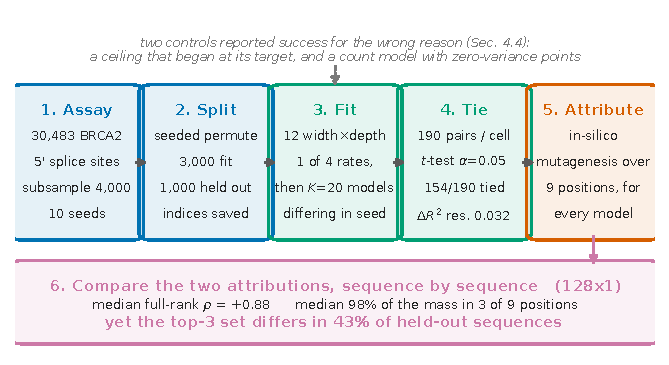
\includegraphics[width=\linewidth]{figures/fig0_workflow.pdf}
  \caption{\textbf{The pipeline, and where the disagreement appears.} Every
  count is read from the committed run behind this paper. Models are trained
  per width $\times$ depth cell differing \emph{only} in initialization seed,
  then filtered to the pairs a paired $t$-test on held-out squared errors
  cannot separate at $\alpha = 0.05$; the surviving pairs are compared by
  in-silico mutagenesis, sequence by sequence. At the best-fitting cell the
  survivors agree well on the full-position ranking and concentrate almost all
  their mass in three positions, yet they disagree about \emph{which} three
  for nearly half of held-out sequences. The two controls named above the
  pipeline both reported success without testing what they were meant to test
  (Section~\ref{sec:why}, Table~\ref{tab:validation}).}
  \label{fig:workflow}
\end{figure}

\section{Problem}

\paragraph{Biological task.}
Given a short RNA sequence and a measured activity, identify \emph{which
positions determine that activity}. In splice-site and siRNA design this is not
a secondary output; it is the object that guides the next round of synthesis. A
designer who reads positions 2, 5 and 6 as critical will vary those and hold the
rest fixed.

\paragraph{Data modality and setting.}
A multiplexed assay of variant effect: each sequence is assayed in a pooled
library and read out as a ratio of two sequencing count pools. We use the BRCA2
exon 17--19 5$'$ splice-site assay of Wong et al.~[9], which quantifies
$\sim$30{,}483 nine-nucleotide sites with $\log_{10}$ percent-spliced-in
readouts and retains per-sequence read counts. We subsample $n = 4000$ per seed,
split 3000 fit / 1000 held out by a fixed seeded permutation recorded with each
run.

\paragraph{Assumption under test.}
That the top-$k$ attributed positions recovered from a well-fitting model are a
property of the sequence--activity relationship rather than of the particular
model that happened to be trained.

\paragraph{Target metric.}
Agreement of the top-$k$ attributed position \emph{set} between models that the
data cannot distinguish on predictive accuracy, measured per-sequence rather
than averaged over the library. We use $k = 3$ throughout, justified in
Section~\ref{sec:why} by the measured concentration of attribution mass and by
Proposition~\ref{prop:rank} in Appendix~\ref{app:formal}.

\paragraph{Desired outcome.}
For the practice to be sound, accuracy-matched models should agree on the top-$k$
set for nearly all sequences. A designer should not get a different answer
because a different seed was used.

\section{Proposed approach}
\label{sec:approach}

The approach under investigation is standard practice~[1,\,8], not a method we
invented: fit a genotype--phenotype model to the assay, compute per-position
attributions by in-silico mutagenesis, and read the top-ranked positions as the
determinants.

\paragraph{Core mechanism.}
A model $f_\theta$ is fit by minimizing predictive loss on the assay.
Attribution scores each position by the mean absolute change in prediction under
substitution, over the real four-letter alphabet:
\begin{equation}
  A_j(x) \;=\; \frac{1}{3}\sum_{b \neq x_j}\bigl|f_\theta(x^{j\to b}) - f_\theta(x)\bigr| .
  \label{eq:ism}
\end{equation}
Positions are ranked by $A_j$ and the top $k$ reported.

\paragraph{Preconditions.}
(i) The model fits the assay well enough that its sensitivities are meaningful.
(ii) The attribution is faithful to the model, in the sense that it reflects the
model's own dependence on each position. (iii) Implicitly, that the model is
\emph{the} model --- that the fitting procedure selects a function determined by
the data.

\paragraph{Hypothesis under which it works.}
If the data determines $f$ up to predictive equivalence, and attribution is
faithful to $f$, then the top-$k$ set is determined by the data. Precondition
(iii) is the one we test, and it is the one that is almost never stated.

\paragraph{Models and protocol.}
Feedforward genotype--phenotype maps over a grid of widths $\{16,32,64,128\}$ and
depths $\{1,2,3\}$, with the per-cell learning rate chosen by pilot on the fit
split. Within a cell we train $K = 20$ models differing \emph{only} in
initialization seed: same architecture, same split, same budget, same learning
rate. All reported quantities use at least 5 seeds with bootstrap intervals;
enumerations are exact and reported as exact. Claims and thresholds were
pre-registered and frozen by a commit hook before the runs
(Appendix~\ref{app:protocol}). Total compute is on the order of GPU-days on a
single mid-range machine.

\section{Observed outcome}

Models the data cannot separate on accuracy assign different top-3 positions for
a large fraction of held-out sequences.

\paragraph{Accuracy matching.}
We filter to pairs whose held-out performance a paired $t$-test on per-point
squared errors cannot separate at $\alpha = 0.05$. This is a failure to reject,
not a demonstration of equivalence, so we report the filter's resolution
alongside it: the minimum detectable held-out $R^2$ difference at 80\% power
given $n_{\text{held-out}} = 1000$. Of 2280 pairs, 1610 are not separable at this
resolution.

\begin{figure}[t]
  \centering
  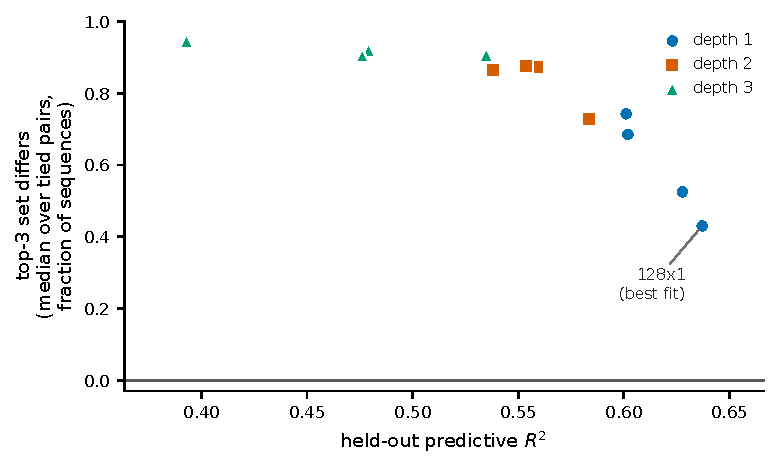
\includegraphics[width=0.86\linewidth]{figures/fig1_not_weak_models.pdf}
  \caption{\textbf{The failure is not an artifact of poorly-fitting models.}
  Each point is one architecture cell: held-out predictive $R^2$ against top-3
  attributed-set divergence between accuracy-matched models. \textbf{The
  plotted quantity is the median, over accuracy-tied pairs, of that pair's
  fraction of held-out sequences whose top-3 sets differ} --- a median over
  pairs of a per-pair fraction, not a single fraction pooled over sequences; the
  same definition is used in Tables~\ref{tab:topk} and~\ref{tab:full}. The
  best-fitting cell still diverges on $43\%$ of sequences, so the failure cannot
  be dismissed as a symptom of underfitting.}
  \label{fig:headline}
\end{figure}

% Generated by experiments/make_tables.py -- do not edit by hand.
\begin{table}[t]
  \caption{\textbf{Models the held-out data cannot tell apart still rank a sequence's positions differently.} Accuracy-tied pairs and their attribution agreement. A pair is \emph{tied} when a paired two-sided $t$-test on per-point held-out squared errors does not reject at $\alpha = 0.05$; \emph{resolution} is the smallest held-out $R^2$ gap that test could have detected at $80\%$ power, so a tie is a failure to reject at a stated resolution rather than a claim of equality. Per-instance $\rho$ is a Spearman correlation between two models' 9-position attribution vectors \emph{for a single held-out sequence}, pooled over sequences and over tied pairs. Bootstrap intervals and the remaining columns are in Table~\ref{tab:full}.}
  \label{tab:tied}
  \centering
  \small
  \begin{tabular}{lrrrrr}
    \toprule
    cell & held-out $R^2$ & tied pairs & resolution ($\Delta R^2$) & $\rho$ p10 / median & frac $\rho<0.5$ \\
    \midrule
    16$\times$1 & 0.6011 & 162/190 & 0.0699 & +0.217 / +0.650 & 30\% \\
    16$\times$2 & 0.5591 & 158/190 & 0.1059 & -0.167 / +0.417 & 58\% \\
    16$\times$3 & 0.5349 & 134/190 & 0.1161 & -0.300 / +0.283 & 69\% \\
    32$\times$1 & 0.6019 & 167/190 & 0.0651 & +0.365 / +0.717 & 19\% \\
    32$\times$2 & 0.5537 & 143/190 & 0.1032 & -0.168 / +0.408 & 58\% \\
    32$\times$3 & 0.4792 & 102/190 & 0.1256 & -0.317 / +0.258 & 71\% \\
    64$\times$1 & 0.6278 & 160/190 & 0.0402 & +0.600 / +0.833 & 4\% \\
    64$\times$2 & 0.5381 & 100/190 & 0.0882 & -0.183 / +0.417 & 57\% \\
    64$\times$3 & 0.3929 & 92/190 & 0.1267 & -0.383 / +0.175 & 78\% \\
    128$\times$1 & 0.6372 & 154/190 & 0.0318 & +0.700 / +0.883 & 2\% \\
    128$\times$2 & 0.5836 & 144/190 & 0.0461 & +0.400 / +0.750 & 16\% \\
    128$\times$3 & 0.4761 & 95/190 & 0.0937 & -0.267 / +0.317 & 67\% \\
    \bottomrule
  \end{tabular}
\end{table}


\paragraph{It is not an artifact of weak models.}
Held-out $R^2$ does correlate with agreement across cells (Spearman $+0.650$
against the minimum $\rho$), so we state the result at the \emph{best}-fitting
cell rather than the worst. At width 128, depth 1 --- held-out $R^2 = 0.637$,
the highest in the grid --- 154 of 190 pairs are accuracy-tied, and among them
37\% rank positions at $\rho$ below 0.9, 15\% below 0.8, and 6\% below 0.7,
reaching $+0.350$ (Figure~\ref{fig:headline}).

\paragraph{The top-$k$ set, which is what gets used.}
The top-3 set differs for 73\% and 90\% of held-out sequences at width 128,
depths 2 and 3; restricted to sequences where the concentration diagnostic
(Section~\ref{sec:why}) says the comparison is meaningful, 71\% and 80\%. The
conditioned figure is reported for completeness but carries little weight at
depth 3: only $11\%$ of sequences at width 128 depth 3 have a well-defined
top-3 under both models, and at width 64 depth 3 none do.
These are accuracy-tied pairs of \emph{independently trained} models, the
population described in Section~\ref{sec:approach}. The corresponding figures
for a fit
against its own reparameterized twin are much smaller --- 46\%, 47\%, 34\% and
21\% --- and are reported separately in Appendix~\ref{gen:twin}; the two
populations must not be quoted interchangeably.

% Generated by experiments/make_tables.py -- do not edit by hand.
\begin{table}[t]
  \caption{\textbf{The disagreement is about which positions carry the mass, not about the ordering of a negligible tail.} Top-3 set agreement and attribution concentration. \emph{top-3 mass} is the median fraction of a sequence's total $|\Delta|$ in its three strongest positions and \emph{effective positions} is $\exp$ of the entropy of the normalized magnitudes, where $9$ means all positions contribute equally. Jaccard on 3-element sets takes only $\{0, 0.2, 0.5, 1\}$, so its median is near-useless as a summary and the \emph{mean} is reported, alongside the fraction of sequences whose top-3 sets match exactly.}
  \label{tab:topk}
  \centering
  \small
  \begin{tabular}{lrrrr}
    \toprule
    cell & top-3 mass & effective positions & top-3 exact match & mean Jaccard \\
    \midrule
    16$\times$1 & 0.926 & 3.03 & 26\% & 0.57 \\
    16$\times$2 & 0.819 & 4.44 & 13\% & 0.43 \\
    16$\times$3 & 0.768 & 5.11 & 9\% & 0.37 \\
    32$\times$1 & 0.956 & 2.56 & 32\% & 0.62 \\
    32$\times$2 & 0.851 & 4.05 & 12\% & 0.42 \\
    32$\times$3 & 0.759 & 5.28 & 8\% & 0.36 \\
    64$\times$1 & 0.969 & 2.36 & 48\% & 0.73 \\
    64$\times$2 & 0.873 & 3.79 & 14\% & 0.43 \\
    64$\times$3 & 0.540 & 7.80 & 6\% & 0.31 \\
    128$\times$1 & 0.976 & 2.20 & 57\% & 0.78 \\
    128$\times$2 & 0.918 & 3.16 & 27\% & 0.60 \\
    128$\times$3 & 0.728 & 5.67 & 10\% & 0.38 \\
    \bottomrule
  \end{tabular}
\end{table}


\paragraph{The data adjudicates cheaply, which sharpens the result rather than
softening it.}
Proposition~\ref{prop:sep} gives the number of
held-out measurements needed to reject that two accuracy-tied models are the
same function, under a noise scale derived from the assay's own read counts
(Proposition~\ref{prop:noise}). For \emph{independently trained} accuracy-tied
pairs the requirement is small in every cell: a median of $0.3$ to $2.1$
measurements, so all twelve cells sit four orders of magnitude below the
$30{,}483$-sequence library (Figure~\ref{fig:sep}). These models are therefore
\emph{easily} distinguishable as functions while being tied on predictive
accuracy, and they still assign different top-3 sets in $43$--$94\%$ of
sequences. The $8.8 \times 10^7$ figure previously quoted here belongs to the
twin comparison (Appendix~\ref{gen:twin}), where the requirement does span nine
orders of magnitude and two cells do exceed the library.

\begin{figure}[t]
  \centering
  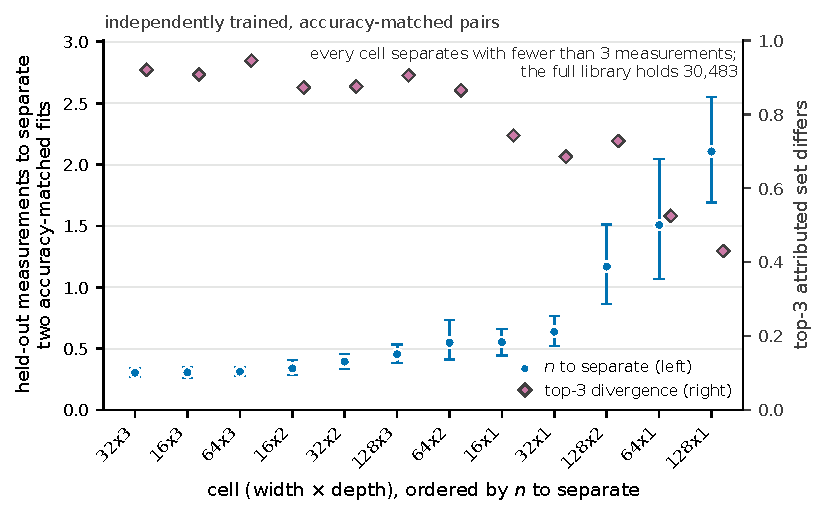
\includegraphics[width=0.86\linewidth]{figures/fig3_occurrence_separability.pdf}
  \caption{\textbf{Accuracy-tied models are cheap to tell apart as functions,
  yet disagree about which positions matter.} Held-out measurements required to
  reject that two \emph{independently trained} accuracy-matched models are the
  same function (Proposition~\ref{prop:sep}), under the assay's own Poisson
  count-noise model, with the top-3 set divergence on the right axis. Every cell
  needs fewer than three measurements, against a library of $30{,}483$, so the
  reference line is off scale and is stated in the panel rather than drawn. The
  companion figure for a fit against its own reparameterized twin, where the
  requirement spans nine orders of magnitude, is Appendix~\ref{gen:twin}.}
  \label{fig:sep}
\end{figure}

\section{Reason for failure}
\label{sec:why}

\subsection{Cause 1: the fitting objective does not identify the attribution}

Predictive loss constrains $f$ on the observed points. It places no constraint on
which of the many equally-accurate functions is selected, and that selection is
made by the initialization seed (Remark~\ref{rem:nonid}). This is the Rashomon
effect~[2,\,3,\,4,\,7] instantiated on a real assay. What is new here is not
that multiplicity exists but its magnitude \emph{at the level of the top-$k$
set}, and the demonstration that the data cannot resolve it.

The consequence is that precondition (iii) of Section~2 is false, and it is the
precondition nobody states. Faithfulness of the attribution to the model
(precondition ii) does not help: a perfectly faithful attribution of an
arbitrarily-selected model is an arbitrary answer.

\subsection{Cause 2: attribution is concentrated, so the usual check cannot detect the failure}

Attribution is not spread evenly across positions. Among accuracy-tied
independently trained pairs, a median 86\% of a sequence's total $|\Delta|$ sits
in its three strongest positions, with an effective 3.9 contributing positions
of 9 by the exponentiated entropy of the normalized magnitudes
(Figure~\ref{fig:concentration}a). The twin comparison gives 82\% and 4.4; the
argument below is unchanged by which is used, but the number quoted must match
the population under discussion.

This is not merely a nuisance; it makes the standard check uninformative, and we
can say by how much. Proposition~\ref{prop:rank} shows that if two models agree
\emph{exactly} on the top 3 of 9 positions and order the remaining 6 at random,
the expected Spearman correlation is $0.708$. A reported $\rho$ of $0.7$ is
therefore consistent with perfect agreement about which positions matter, and
also with substantial disagreement. The statistic cannot distinguish the two.

\begin{figure}[t]
  \centering
  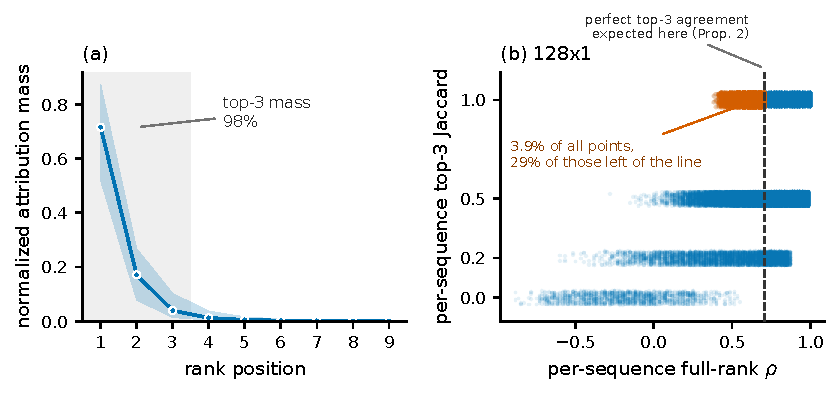
\includegraphics[width=0.98\linewidth]{figures/fig2_concentration.pdf}
  \caption{\textbf{A low rank correlation has two incompatible readings, and the
  top-$k$ set separates them.} Accuracy-tied independently trained pairs at
  width 128, depth 1; three seeds, $203{,}200$ (sequence, pair) points.
  (a) Normalized attribution mass by rank position, median over $24{,}000$
  held-out sequence profiles with interquartile band: a median $97\%$ of the
  mass sits in the top three positions and the remainder collapses to near
  zero. (b) Per-sequence full-rank $\rho$ against per-sequence top-3 set
  Jaccard. The dashed line is $\rho = 0.708$, the value Proposition~\ref{prop:rank}
  gives for two models that agree \emph{exactly} on the top 3 and order the
  remaining 6 at random. Points left of it with Jaccard $= 1$ (highlighted) are
  cases where the two models pick the same three positions while the rank
  correlation reads as disagreement. \textbf{There are $8{,}861$ such
  (sequence, pair) observations: $4.4\%$ of all $203{,}200$ plotted, and
  $30\%$ of the $29{,}310$ that fall left of the line.} Each observation is one
  held-out sequence under one accuracy-tied pair, so the region is a substantial
  population rather than a handful of outliers. The statistic cannot distinguish
  the two readings; the top-$k$ set can.}
  \label{fig:concentration}
\end{figure}

\paragraph{Diagnostic.}
Report the top-$k$ position \emph{set} overlap and the concentration alongside
it. Under that diagnostic, ten of twelve cells show genuine disagreement about
which positions matter, and it does so in every cell of the grid. Exact top-3
agreement runs 26--57\% at depth 1, 12--27\% at depth 2 and 6--10\% at depth 3.
The best cell in the grid, width 128 depth 1, still assigns a different top-3
set for $43\%$ of held-out sequences. We had expected a low-capacity exemption
and there is none: the smallest models are among the \emph{worst}, not the
best. See Section~\ref{sec:boundary}.

\subsection{Cause 3: the noise model, and a silent failure in ours}

Asking how much data would separate two models requires a noise scale, and this
assay supplies one rather than needing an assumption. The phenotype is affine in
$\log_{10}$ of a count ratio: regressing $y$ on $\log_{10}(\text{ex}/\text{tot})$
over the library gives slope $0.933$ with $r = 0.990$. Those are two independent
count pools, not a proportion --- \text{ex} exceeds \text{tot} in 4.9\% of rows,
by up to $20.9\times$ --- so a binomial model is wrong here.
Proposition~\ref{prop:noise} gives the Poisson log-ratio scale.

\paragraph{Our first noise model failed silently, in the direction that hides the
result.}
Under a binomial form, a near-saturated sequence receives $\sigma \to 0$; since
the separation test of Proposition~\ref{prop:sep} weights points by
$1/\sigma^2$, a handful of such points dominated and the required sample size
collapsed to zero --- that is, the analysis reported that the models were
trivially separable. The binomial model is also inapplicable on its own terms
here: $N_{\mathrm{ex}} \ge N_{\mathrm{tot}}$ on $4.9\%$ of rows, where the
binomial variance is zero or negative. Under the Poisson log-ratio the weight
distribution is unremarkable --- the mean of $1/\sigma^2$ is $3.0$ times its
median --- and the requirement becomes meaningful. We do not quote a magnitude
for the binomial inflation: that model was replaced before the separation
experiment was first committed, so the figure cannot be regenerated from
released code (Appendix~\ref{gen:noise}). Counting noise is a lower bound on
total noise, so every reported requirement is a lower bound.

\subsection{Cause 4: two ways our validation nearly hid the failure}

Both are errors we committed and caught. We report them because the controls that
catch them are cheap and appear not to be standard. Table~\ref{tab:validation}
states each one as what was reported, what was actually tested, and what the
corrected check reports.

% Generated by experiments/make_tables.py -- do not edit by hand.
\begin{table}[t]
  \caption{\textbf{Both controls we relied on were passing for reasons unrelated to what they were meant to test.} Each row is a check that reported a clean result, the property it actually verified, and what the corrected check reports. Neither failure was visible from the reported number alone: a control that cannot fail and a weighting scheme that silently concentrates on a few points both look like success.}
  \label{tab:validation}
  \centering
  \small
  \begin{tabular}{p{0.10\linewidth}p{0.24\linewidth}p{0.30\linewidth}p{0.28\linewidth}}
    \toprule
    check & what it reported & what it actually tested & corrected control \\
    \midrule
    \textbf{Ceiling control} & Held-out $R^2 = 1.000000$ recovering a target the architecture realizes exactly, in every cell and every seed. & That Adam does not leave a perfect solution. The refit was warm-started \emph{at} the target, its initial loss was already below the stopping threshold, and best-iterate selection kept the initial state, so the optimization loop never ran. & Cold-started on the same in-class target, the worst cell reaches only $0.4501$ ($64\times3$) and 11 of 12 cells fall below the $0.999$ threshold. \\
    \textbf{Noise model} & A required sample size of zero: any two fits separable with no data at all. & Inverse-variance weighting under a count model that is undefined on this library. The two pools are not a proportion --- $\mathrm{ex} \ge \mathrm{tot}$ on $4.9\%$ of rows --- so the binomial variance is zero or negative there and a handful of near-saturated sequences carried the whole statistic. & Under the Poisson log-ratio the weight distribution is ordinary (mean $1/\sigma^2$ is $3.0$ times its median) and the requirement becomes finite and cell-dependent, spanning $0.5$ to $87{,}751{,}464$ measurements. \\
    \bottomrule
  \end{tabular}
\end{table}


\paragraph{A ceiling that was arithmetic, not evidence.}
To check that a refit procedure can recover a target, one refits to a target the
model class provably contains and confirms recovery. Our implementation
warm-started the refit from the reference weights. For the null target --- the
reference's own latent --- the initial loss was already $6.7 \times 10^{-19}$,
below the early-stopping threshold, so best-iterate selection kept the initial
state and the optimization loop never ran. The control returned $1.000000$
because it \emph{began at the answer}. It verified that the optimizer does not
wander away from a perfect solution; it never verified that the procedure can
\emph{find} a solution it does not start at, which is the capability every
downstream conclusion assumed. Details in Appendix~\ref{app:ceiling}.

The fix is a ceiling that requires search: cold-start the same refit. Under that
control, recovery of a target the architecture realizes \emph{exactly} falls to
held-out $R^2 \approx 0.45$ at depth 3, with per-seed variation indicating
distinct basins rather than measurement noise.

\paragraph{A negative reported from an empty search.}
A separate experiment reported ``no witness found'' after examining zero
candidates: every cell it searched had an empty candidate set for structural
reasons. Searched-and-found-nothing is a result; never-searched is not, and the
second was reported as the first. We now emit a \textsc{void} verdict whenever a
negative would be drawn from an empty candidate set, with a regression test
pinning the distinction.

\subsection{Boundary conditions}
\label{sec:boundary}

The practice is not always unsound, and the conditions are measurable.

\begin{itemize}
\item \textbf{Depth is what tracks the failure; width is not, and no cell is
  safe.} Top-3 divergence rises monotonically with depth: $43$--$74\%$ at depth
  1, $73$--$88\%$ at depth 2, $90$--$94\%$ at depth 3, a rank correlation of
  $+0.80$ with depth against $-0.06$ with width. Within depth 1 it improves with
  width, from $74\%$ at width 16 to $43\%$ at width 128, but it never falls
  below $43\%$ anywhere in the grid. We looked for a low-capacity exemption and
  found the opposite: the narrowest models are among the worst.
\item \textbf{It degrades with capacity, not with fit quality alone.} The
  correlation between held-out $R^2$ and agreement is $+0.650$: real, but far
  from explanatory, and the best-fitting cell still shows the failure.
\item \textbf{Pairs that are harder to tell apart agree more, not less.} Across
  cells the median number of held-out measurements needed to separate a tied
  pair as functions is rank-correlated $-0.94$ with top-3 divergence: where the
  two fits are closer as functions they also pick more similar positions, which
  is the direction one would want and the opposite of what the twin comparison
  shows (Appendix~\ref{gen:twin}). The failure is therefore not a by-product of
  the two fits being nearly identical.
\item \textbf{Scope.} One assay, one phenotype, sequence length 9. We do not
  claim this generalizes to longer contexts or to models with strong
  architectural priors, and we tested only in-silico mutagenesis, not gradient
  or Shapley-based attribution.
\end{itemize}

\subsection{Actionable takeaways}

\begin{enumerate}
\item \textbf{Report per-instance top-$k$ sets, not a library-averaged rank
  correlation.} By Proposition~\ref{prop:rank} the averaged correlation cannot
  distinguish perfect agreement from substantial disagreement.
\item \textbf{Report the concentration of the attribution.} Without it a reader
  cannot interpret a rank correlation at all, because the reference value under
  perfect agreement depends on it.
\item \textbf{Derive the noise scale from the assay where counts are available},
  and check the count model. Ours was wrong in the direction that made the
  problem disappear.
\item \textbf{Train more than one seed and report top-$k$ set agreement across
  them.} This costs a constant factor and is the single cheapest check that would
  have caught the failure.
\item \textbf{Verify that a passing control required a search.} A control that
  starts at its own target passes by arithmetic.
\item \textbf{Refuse to report a negative from an empty candidate set.}
\end{enumerate}

\section*{References}

\medskip
{
\small

[1] Alipanahi, B., Delong, A., Weirauch, M.T.\ \& Frey, B.J.\ (2015) Predicting
the sequence specificities of DNA- and RNA-binding proteins by deep learning.
{\it Nature Biotechnology} {\bf 33}(8):831--838.

[2] Breiman, L.\ (2001) Statistical modeling: the two cultures. {\it Statistical
Science} {\bf 16}(3):199--231.

[3] Fisher, A., Rudin, C.\ \& Dominici, F.\ (2019) All models are wrong, but many
are useful: learning a variable's importance by studying an entire class of
prediction models simultaneously. {\it Journal of Machine Learning Research}
{\bf 20}(177):1--81.

[4] Hsu, H.\ \& Calmon, F.P.\ (2022) Rashomon capacity: a metric for predictive
multiplicity in classification. In {\it Advances in Neural Information
Processing Systems 35}, pp.\ 28988--29000.

[5] Marx, C., Calmon, F.\ \& Ustun, B.\ (2020) Predictive multiplicity in
classification. In {\it Proceedings of the 37th International Conference on
Machine Learning}, PMLR {\bf 119}:6765--6774.

[6] Seitz, E.E., McCandlish, D.M., Kinney, J.B.\ \& Koo, P.K.\ (2024)
Interpreting cis-regulatory mechanisms from genomic deep neural networks using
surrogate models. {\it Nature Machine Intelligence} {\bf 6}:701--713.

[7] Semenova, L., Rudin, C.\ \& Parr, R.\ (2022) On the existence of simpler
machine learning models. In {\it Proceedings of the 2022 ACM Conference on
Fairness, Accountability, and Transparency}, pp.\ 1827--1858.

[8] Tareen, A., Kooshkbaghi, M., Posfai, A., Ireland, W.T., McCandlish, D.M.\ \&
Kinney, J.B.\ (2022) MAVE-NN: learning genotype--phenotype maps from multiplex
assays of variant effect. {\it Genome Biology} {\bf 23}:98.

[9] Wong, M.S., Kinney, J.B.\ \& Krainer, A.R.\ (2018) Quantitative activity
profile and context dependence of all human 5$'$ splice sites. {\it Molecular
Cell} {\bf 71}(6):1012--1026.

[10] Zhou, S., Huang, M.\ \& Li, K.\ (2026) Position: genomic model research must
move beyond anecdotal evaluation of interpretability methods. In {\it Proceedings
of the 43rd International Conference on Machine Learning}. arXiv:2606.07607.

}

\appendix

\section{Formal statements}
\label{app:formal}

The statements below are elementary. We give them explicitly because two of
them (Propositions~\ref{prop:rank} and~\ref{prop:noise}) determine how the
main-text numbers should be read, and because the failure described in
Section~4.3 was a violation of Proposition~\ref{prop:noise} that produced a
plausible-looking wrong answer rather than an error.

\begin{remark}[Predictive risk does not determine the attribution]
\label{rem:nonid}
Let $\mathcal{F}$ be a model class, $R$ a population risk, and
$\mathcal{F}_\epsilon = \{f \in \mathcal{F} : R(f) \le \min_{f'} R(f') + \epsilon\}$
the $\epsilon$-Rashomon set. Let $A : \mathcal{F} \to \mathbb{R}^L$ be the
attribution map of Eq.~\eqref{eq:ism}. Nothing in the definition of
$\mathcal{F}_\epsilon$ constrains $A$ to be constant on it. Consequently, the
attribution reported by a fitting procedure is a function of \emph{which}
element of $\mathcal{F}_\epsilon$ the optimizer returns, and that is determined
by the initialization, not by the data. The empirical content of this paper is
the diameter of $A(\mathcal{F}_\epsilon)$ on a real assay, measured at the level
of the top-$k$ set.
\end{remark}

\begin{proposition}[Expected rank correlation under concentrated attribution]
\label{prop:rank}
Let two models rank $L$ positions. Suppose they agree exactly on the ordering of
the top $k$ positions, and that the remaining $m = L - k$ positions carry
negligible attribution mass, so that their relative orderings are independent
uniform random permutations. Then the expected Spearman rank correlation over
all $L$ positions is
\begin{equation}
  \mathbb{E}[\rho_L] \;=\; 1 - \frac{m(m^2 - 1)}{L(L^2 - 1)} .
\end{equation}
For $L = 9$ and $k = 3$ this is $1 - \nicefrac{210}{720} = 0.708$.
\end{proposition}

\begin{proof}
Spearman's $\rho$ over $L$ items is
$\rho = 1 - 6\sum_i d_i^2 / \bigl(L(L^2-1)\bigr)$, where $d_i$ is the rank
difference at item $i$. The top $k$ contribute $d_i = 0$ by assumption. For two
independent uniform permutations of $m$ items, $\mathbb{E}[\rho_m] = 0$, and
since $\rho_m = 1 - 6\sum d_i^2/\bigl(m(m^2-1)\bigr)$ this gives
$\mathbb{E}\bigl[\sum d_i^2\bigr] = m(m^2-1)/6$ over the tail block.
Substituting yields the result.
\end{proof}

\begin{table}[h]
  \caption{Expected Spearman correlation over $L = 9$ positions when two models
  agree \emph{exactly} on the top $k$ and order the rest at random
  (Proposition~\ref{prop:rank}). A reported $\rho$ at or below these values
  carries no evidence of disagreement about which positions matter.}
  \label{tab:rho-null}
  \centering
  \small
  \begin{tabular}{lrrrr}
    \toprule
    top-$k$ agreed & $k=2$ & $k=3$ & $k=4$ & $k=5$ \\
    \midrule
    $\mathbb{E}[\rho_9]$ & 0.533 & 0.708 & 0.833 & 0.917 \\
    \bottomrule
  \end{tabular}
\end{table}

\begin{proposition}[Poisson log-ratio noise scale]
\label{prop:noise}
Let the phenotype be $y = a\log_{10}(N_{\mathrm{ex}}/N_{\mathrm{tot}}) + b$ with
$N_{\mathrm{ex}}$ and $N_{\mathrm{tot}}$ independent Poisson counts with means
$\lambda_{\mathrm{ex}}, \lambda_{\mathrm{tot}}$. Then to first order
\begin{equation}
  \mathrm{sd}(y) \;=\; \frac{|a|}{\ln 10}
  \sqrt{\frac{1}{\lambda_{\mathrm{ex}}} + \frac{1}{\lambda_{\mathrm{tot}}}}
  \;\;\approx\;\; \frac{|a|}{\ln 10}
  \sqrt{\frac{1}{N_{\mathrm{ex}}} + \frac{1}{N_{\mathrm{tot}}}} .
\end{equation}
\end{proposition}

\begin{proof}
For $N \sim \mathrm{Poisson}(\lambda)$, the delta method with $g(N) = \ln N$
gives $\mathrm{Var}(\ln N) \approx \lambda^{-2}\mathrm{Var}(N) = 1/\lambda$.
Independence of the two pools gives
$\mathrm{Var}(\ln N_{\mathrm{ex}} - \ln N_{\mathrm{tot}}) \approx
1/\lambda_{\mathrm{ex}} + 1/\lambda_{\mathrm{tot}}$. Converting to base 10 and
scaling by $a$ yields the result; substituting counts for means is the usual
plug-in estimator.
\end{proof}

\begin{remark}[Why the binomial form fails here, and fails silently]
Modelling the readout as a proportion $p$ from $N$ trials gives
$\mathrm{sd}(y) \propto \sqrt{(1-p)/(Np)}$, which tends to $0$ as $p \to 1$.
Since the statistic of Proposition~\ref{prop:sep} weights points by
$1/\sigma_i^2$, a small number of near-saturated sequences then carry unbounded
weight. Under Proposition~\ref{prop:noise} the ratio
$\mathrm{mean}(1/\sigma^2)/\mathrm{median}(1/\sigma^2)$ is $3.0$, a heavy but
unremarkable tail. We give no corresponding figure for the binomial form: it was
replaced before the separation experiment was first committed and cannot be
regenerated from released code, so only the structural defect is quoted. That
defect is decisive on its own: $N_{\mathrm{ex}} > N_{\mathrm{tot}}$ in 4.9\% of
rows, by up to $20.9\times$, so the two counts are not numerator and
denominator of a proportion.
\end{remark}

\begin{proposition}[Separation sample size]
\label{prop:sep}
Let $f_1, f_2$ be two candidate functions with pointwise difference
$d_i = f_1(x_i) - f_2(x_i)$ at held-out points $x_i$, and let observations carry
independent Gaussian noise with known standard deviations $\sigma_i$. Testing
$H_0 : y \sim f_1$ against $H_1 : y \sim f_2$ at two-sided level $\alpha$ with
power $1 - \beta$ requires
\begin{equation}
  n \;\ge\; \frac{\bigl(z_{1-\alpha/2} + z_{1-\beta}\bigr)^2}
  {\overline{\left(d_i / \sigma_i\right)^2}} ,
  \qquad
  \overline{\left(d_i/\sigma_i\right)^2}
  \;=\; \frac{1}{n}\sum_{i=1}^{n} \frac{d_i^2}{\sigma_i^2} .
\end{equation}
\end{proposition}

\begin{proof}
The log-likelihood ratio between the two simple hypotheses is Gaussian with mean
$\pm\tfrac12\sum_i d_i^2/\sigma_i^2$ under $H_0$ and $H_1$ respectively, and
variance $\sum_i d_i^2/\sigma_i^2$. The standardized separation is therefore
$\bigl(\sum_i d_i^2/\sigma_i^2\bigr)^{1/2}$, and the standard two-sided power
requirement $\bigl(\sum_i d_i^2/\sigma_i^2\bigr)^{1/2} \ge z_{1-\alpha/2} + z_{1-\beta}$
rearranges to the stated bound.
\end{proof}

\begin{remark}[The reported requirement is a lower bound]
Proposition~\ref{prop:noise} accounts for sequencing count noise only. Library
preparation, transfection and biological variation add further variance, which
increases $\sigma_i$ and hence increases the required $n$. Every separation
requirement in the main text is therefore a lower bound on the measurements
needed.
\end{remark}

\begin{proposition}[Effective number of contributing positions]
\label{prop:eff}
For an attribution vector $A \in \mathbb{R}_{\ge 0}^L$ with $\sum_j A_j > 0$, let
$q_j = A_j / \sum_{j'} A_{j'}$. The effective number of contributing positions is
$N_{\mathrm{eff}}(A) = \exp\bigl(-\sum_j q_j \ln q_j\bigr)$, satisfying
$1 \le N_{\mathrm{eff}} \le L$, with $N_{\mathrm{eff}} = L$ iff all positions
contribute equally and $N_{\mathrm{eff}} \to 1$ as one position dominates.
\end{proposition}

\noindent This is the exponentiated Shannon entropy of the normalized attribution
and is reported per-sequence in Table~\ref{tab:topk}; the median over held-out
sequences is $3.9$ of $9$ for accuracy-tied
independently trained pairs, and $4.4$ of $9$ for the twin comparison.

\section{Full per-cell results}
\label{app:full}

Table~\ref{tab:full} combines Tables~\ref{tab:tied} and~\ref{tab:topk} for
every cell in the width $\times$ depth grid, with bootstrap intervals on the
columns that admit them. It is generated by
\texttt{experiments/make\_tables.py} directly from the committed run
directories, as are all tables in this paper.

% Generated by experiments/make_tables.py -- do not edit by hand.
\begin{table}[!htb]
  \centering
  \small
  \resizebox{\ifdim\width>\linewidth\linewidth\else\width\fi}{!}{%
  \begin{tabular}{lllrrrrrrrr}
    \toprule
    cell & held-out $R^2$ & tied pairs & res.\ & $\rho$ p10 / med & $\rho{<}0.5$ & top-3 mass & eff.\ pos & top-1 diff & exact & Jaccard \\
    \midrule
    16$\times$1 & 0.6011 \tiny[0.5725, 0.6274] & 162 \tiny[156, 169] & 0.0699 & +0.217 / +0.650 & 30\% & 0.926 & 3.03 & 45\% & 26\% & 0.57 \\
    16$\times$2 & 0.5591 \tiny[0.5243, 0.5880] & 158 \tiny[147, 167] & 0.1059 & -0.167 / +0.417 & 58\% & 0.819 & 4.44 & 60\% & 13\% & 0.43 \\
    16$\times$3 & 0.5349 \tiny[0.4948, 0.5677] & 134 \tiny[122, 147] & 0.1161 & -0.300 / +0.283 & 69\% & 0.768 & 5.11 & 68\% & 9\% & 0.37 \\
    32$\times$1 & 0.6019 \tiny[0.5754, 0.6263] & 167 \tiny[160, 172] & 0.0651 & +0.365 / +0.717 & 19\% & 0.956 & 2.56 & 37\% & 32\% & 0.62 \\
    32$\times$2 & 0.5537 \tiny[0.5110, 0.5909] & 143 \tiny[128, 158] & 0.1032 & -0.168 / +0.408 & 58\% & 0.851 & 4.05 & 62\% & 12\% & 0.42 \\
    32$\times$3 & 0.4792 \tiny[0.4128, 0.5349] & 102 \tiny[97, 108] & 0.1256 & -0.317 / +0.258 & 71\% & 0.759 & 5.28 & 69\% & 8\% & 0.36 \\
    64$\times$1 & 0.6278 \tiny[0.6003, 0.6544] & 160 \tiny[151, 169] & 0.0402 & +0.600 / +0.833 & 4\% & 0.969 & 2.36 & 24\% & 48\% & 0.73 \\
    64$\times$2 & 0.5381 \tiny[0.4846, 0.5861] & 100 \tiny[81, 120] & 0.0882 & -0.183 / +0.417 & 57\% & 0.873 & 3.79 & 61\% & 14\% & 0.43 \\
    64$\times$3 & 0.3929 \tiny[0.3309, 0.4483] & 92 \tiny[86, 97] & 0.1267 & -0.383 / +0.175 & 78\% & 0.540 & 7.80 & 74\% & 6\% & 0.31 \\
    128$\times$1 & 0.6372 \tiny[0.6122, 0.6585] & 154 \tiny[138, 166] & 0.0318 & +0.700 / +0.883 & 2\% & 0.976 & 2.20 & 18\% & 57\% & 0.78 \\
    128$\times$2 & 0.5836 \tiny[0.5369, 0.6259] & 144 \tiny[119, 168] & 0.0461 & +0.400 / +0.750 & 16\% & 0.918 & 3.16 & 36\% & 27\% & 0.60 \\
    128$\times$3 & 0.4761 \tiny[0.3949, 0.5456] & 95 \tiny[71, 117] & 0.0937 & -0.267 / +0.317 & 67\% & 0.728 & 5.67 & 68\% & 10\% & 0.38 \\
    \bottomrule
  \end{tabular}}
  \caption{\textbf{No cell is withheld: the pattern in Tables~\ref{tab:tied} and~\ref{tab:topk} holds across the whole grid.} All twelve cells, combining both main-text tables. \textbf{Which columns carry intervals, and why the rest do not:} held-out $R^2$ and the tied-pair count are per-seed quantities and are given as mean with a $95\%$ bootstrap interval over the ten seeds. The remaining columns are medians pooled over every tied pair across all seeds rather than per-seed values, so a seed-level bootstrap interval is not defined for them and none is invented here.}
  \label{tab:full}
\end{table}


\section{Protocol and pre-registration}
\label{app:protocol}

Table~\ref{tab:protocol} gives the per-cell protocol, read from the
\texttt{tuning\_budget.json} written with each run and from the per-seed
records. The split rule is the same everywhere: for seed $k$ a generator seeded
with $1{,}000{,}003 + k$ draws a permutation of the $4000$ subsampled sequences,
the first $3000$ form the fit split and the remaining $1000$ are held out, and
the indices are recorded in the run directory. All twelve cells use ten seeds.

% Generated by experiments/make_tables.py -- do not edit by hand.
\begin{table}[!htb]
  \centering
  \small
  \resizebox{\ifdim\width>\linewidth\linewidth\else\width\fi}{!}{%
  \begin{tabular}{lllrr}
    \toprule
    cell & learning rate chosen (seeds) & configs & epochs & grad.\ steps \\
    \midrule
    16$\times$1 & 0.01 & 4 & 1,200 & 1,200 \\
    16$\times$2 & 0.01 & 4 & 1,200 & 1,200 \\
    16$\times$3 & 0.01 ($\times$9), 0.003 ($\times$1) & 4 & 1,200 & 1,200 \\
    32$\times$1 & 0.01 & 4 & 1,200 & 1,200 \\
    32$\times$2 & 0.01 & 4 & 1,200 & 1,200 \\
    32$\times$3 & 0.01 & 4 & 1,200 & 1,200 \\
    64$\times$1 & 0.01 ($\times$4), 0.003 ($\times$6) & 4 & 1,200 & 1,200 \\
    64$\times$2 & 0.01 ($\times$9), 0.003 ($\times$1) & 4 & 1,200 & 1,200 \\
    64$\times$3 & 0.01 ($\times$9), 0.003 ($\times$1) & 4 & 1,200 & 1,200 \\
    128$\times$1 & 0.003 ($\times$9), 0.001 ($\times$1) & 4 & 1,200 & 1,200 \\
    128$\times$2 & 0.003 ($\times$4), 0.001 ($\times$6) & 4 & 1,200 & 1,200 \\
    128$\times$3 & 0.003 ($\times$4), 0.001 ($\times$6) & 4 & 1,200 & 1,200 \\
    \bottomrule
  \end{tabular}}
  \caption{\textbf{The tuning budget is four learning rates per cell and nothing else, so the disagreement cannot be an artifact of unequal search.} Per-cell protocol, read from \texttt{tuning\_budget.json} and the per-seed records. The search space is ``learning rate over [0.01, 0.003, 0.001, 0.0003], selected once per cell and shared by all models in it''. The selection rule is identical in every cell --- ``no model selection: every trained model is kept and enters the pairwise analysis'' --- so it is stated here rather than repeated as a column. \textbf{The chosen rate is not constant across seeds:} it varies in 7 of 12 cells, and the multiplicities are given. Within any one seed a single rate is shared by all 20 models in the cell, so the models still differ only in initialization; across seeds the rate is re-selected.}
  \label{tab:protocol}
\end{table}


Claims, thresholds and go/no-go criteria were written and committed before any
result existed: \texttt{PREREGISTRATION.md} has a single commit, dated
2026-08-26, and the earliest committed run directory is dated 2026-08-29, so
the ordering is checkable from the repository history rather than asserted.
Amendment is additionally blocked by a pre-write hook in the authoring
environment that matches the target path of a write; we name the mechanism
precisely because it constrains our workflow rather than the repository, and
the durable evidence is the single-commit history. Every reported number
carries the git SHA and configuration hash of the run that produced it.

\section{The vacuous ceiling, in full}
\label{app:ceiling}

The refit loads the reference weights, then evaluates the loss and snapshots
the best iterate \emph{before} entering the optimization loop. For the null
target --- the reference's own latent --- that initial state is already the
best iterate that will ever be seen, so no later step can displace it. The
measured initial loss is $6.7 \times 10^{-19}$, below the $10^{-10}$
early-stopping threshold, and the loop breaks on its first iteration.

The consequence is visible in the run records without reference to any loss
value: the warm-started control returns held-out $R^2$ of exactly $1.0$ in all
$120$ cell--seed combinations, bit-exact rather than approximate. A control
that cannot return anything else has not measured anything. The cold-started
replacement, which must actually travel to the same in-class target, recovers
it at only $0.4501$ in the worst cell and falls below the $0.999$ threshold in
11 of 12 cells, with per-seed spread of $0.21$ to $0.87$ at width 128 depth 3.
Both arms are plotted in Figure~\ref{gen:ceiling-fig}.

The general form of the error is worth stating separately from its instance. A
control that verifies a procedure can recover a target must ensure the procedure
does not \emph{begin} at that target. Warm-starting a refit from the reference
weights and then asking it to recover the reference's own output satisfies the
letter of the control and none of its purpose.

\section{Reproducibility}
\label{app:repro}

Code, pre-registered analysis plans, per-seed raw values, and run provenance are
released at \url{https://github.com/shadi97kh/CERTGNN}. Each result directory
records the git SHA, the configuration hash, the seed list, and the tuning
budget consumed, and every table and figure in this paper is generated from
those directories by \texttt{experiments/make\_tables.py},
\texttt{make\_figures.py} and \texttt{make\_workflow\_figure.py} rather than
transcribed.

% Supplementary material the appendix above does not already cover:
% the noise-model derivation, the twin comparison, and cold-start recovery.
% No second \appendix -- one has already been issued above.
% Generated by experiments/make_appendix.py -- do not edit by hand.
% Every number is read from a committed run record at generation time.
% Requires: booktabs, amsmath, url, hyperref, graphicx.
% Labels are namespaced gen:* so they cannot collide with the
% author's own app:* appendix labels in the main file.

\section{Full per-cell results}
\label{gen:cells}

The main text reports a subset of cells. Both grids are given here in full, all twelve cells, as mean with a 95\% bootstrap confidence interval over 10 seeds. No row is omitted and no cell is excluded.

\subsection{Occurrence grid}

Run \texttt{20260830T002223Z\_6f98de3\_6e25cf7d}, git \texttt{6f98de3}, config \texttt{6e25cf7d}. 4000 sequences per seed, 3000 fit and 1000 held out, 20 models per cell differing only in initialization seed. A pair is \emph{indistinguishable} when a paired two-sided $t$-test on per-point held-out squared errors does not reject at $\alpha = 0.05$; all pooled statistics below are taken over indistinguishable pairs only.

\begin{table}[h]
\centering
\small
\begin{tabular}{llrlrrrr}
\toprule
width & depth & params & held-out $R^2$ & indist. & median $\rho$ & top-3 exact & top-3 Jaccard \\
\midrule
16 & 1 & 609 & 0.6011 \small[0.5725, 0.6274] & 162/190 & +0.917 & 26\% & 0.57 \\
16 & 2 & 881 & 0.5591 \small[0.5243, 0.5880] & 158/190 & +0.833 & 13\% & 0.43 \\
16 & 3 & 1,153 & 0.5349 \small[0.4948, 0.5677] & 134/190 & +0.817 & 9\% & 0.37 \\
32 & 1 & 1,217 & 0.6019 \small[0.5754, 0.6263] & 167/190 & +0.917 & 32\% & 0.62 \\
32 & 2 & 2,273 & 0.5537 \small[0.5110, 0.5909] & 143/190 & +0.817 & 12\% & 0.42 \\
32 & 3 & 3,329 & 0.4792 \small[0.4128, 0.5349] & 102/190 & +0.833 & 8\% & 0.36 \\
64 & 1 & 2,433 & 0.6278 \small[0.6003, 0.6544] & 160/190 & +0.933 & 48\% & 0.73 \\
64 & 2 & 6,593 & 0.5381 \small[0.4846, 0.5861] & 100/190 & +0.850 & 14\% & 0.43 \\
64 & 3 & 10,753 & 0.3929 \small[0.3309, 0.4483] & 92/190 & +0.900 & 6\% & 0.31 \\
128 & 1 & 4,865 & 0.6372 \small[0.6122, 0.6585] & 154/190 & +0.933 & 57\% & 0.78 \\
128 & 2 & 21,377 & 0.5836 \small[0.5369, 0.6259] & 144/190 & +0.883 & 27\% & 0.60 \\
128 & 3 & 37,889 & 0.4761 \small[0.3949, 0.5456] & 95/190 & +0.833 & 10\% & 0.38 \\
\bottomrule
\end{tabular}
\caption{Occurrence grid, all twelve cells. \emph{indist.} is the mean number of accuracy-indistinguishable pairs out of all pairs. \emph{median $\rho$} is the median per-instance Spearman correlation between the two models' per-position attribution magnitudes. \emph{top-3 exact} is the median over indistinguishable pairs of that pair's fraction of held-out sequences whose top-3 attributed sets match exactly, so it is a median over pairs of a per-pair fraction rather than a single pooled fraction over sequences.}
\end{table}

\subsection{Separation grid}

Run \texttt{20260830T030657Z\_972496a\_5da8cb38}, git \texttt{972496a}, config \texttt{5da8cb38}. Same library and split as above, sequence length 9. $Z$ is the number of held-out measurements needed to reject that a fit and its reparameterized twin are the same function, at $\alpha = 0.05$ with power 0.8, under the noise model of Appendix~\ref{gen:noise}.

\begin{table}[h]
\centering
\small
\begin{tabular}{llrllrr}
\toprule
width & depth & params & held-out $R^2$ & per-instance median $\rho$ & $Z$ to separate & top-3 exact \\
\midrule
16 & 1 & 609 & 0.984087 \small[0.979785, 0.987518] & 0.892 \small[0.877, 0.903] & 1 \small[0, 1] & 56\% \\
16 & 2 & 881 & 0.999241 \small[0.998708, 0.999619] & 0.978 \small[0.973, 0.983] & 42 \small[25, 60] & 82\% \\
16 & 3 & 1,153 & 0.999583 \small[0.999138, 0.999916] & 0.984 \small[0.978, 0.990] & 313 \small[87, 571] & 86\% \\
32 & 1 & 1,217 & 0.992155 \small[0.990567, 0.993674] & 0.872 \small[0.847, 0.893] & 0 \small[0, 1] & 48\% \\
32 & 2 & 2,273 & 0.997328 \small[0.995451, 0.999059] & 0.915 \small[0.892, 0.937] & 87 \small[14, 193] & 61\% \\
32 & 3 & 3,329 & 0.999166 \small[0.998775, 0.999529] & 0.923 \small[0.898, 0.945] & 833 \small[18, 2,136] & 61\% \\
64 & 1 & 2,433 & 0.998324 \small[0.997555, 0.998958] & 0.899 \small[0.886, 0.913] & 2 \small[1, 3] & 53\% \\
64 & 2 & 6,593 & 0.999997 \small[0.999995, 0.999998] & 0.855 \small[0.832, 0.880] & 4,176 \small[1,320, 7,333] & 48\% \\
64 & 3 & 10,753 & 0.999996 \small[0.999993, 0.999998] & 0.847 \small[0.835, 0.860] & 7,300 \small[2,156, 14,436] & 43\% \\
128 & 1 & 4,865 & 0.999876 \small[0.999862, 0.999889] & 0.923 \small[0.913, 0.933] & 9 \small[7, 11] & 54\% \\
128 & 2 & 21,377 & 1.000000 \small[1.000000, 1.000000] & 0.905 \small[0.888, 0.920] & 3,158,529 \small[1,402,633, 5,004,083] & 54\% \\
128 & 3 & 37,889 & 1.000000 \small[1.000000, 1.000000] & 0.890 \small[0.885, 0.895] & 87,751,464 \small[39,140,215, 138,392,840] & 53\% \\
\bottomrule
\end{tabular}
\caption{Separation grid, all twelve cells. $Z$ is a lower bound: it counts sequencing noise only (Appendix~\ref{gen:noise}).}
\end{table}

\begin{figure}[h]
\centering
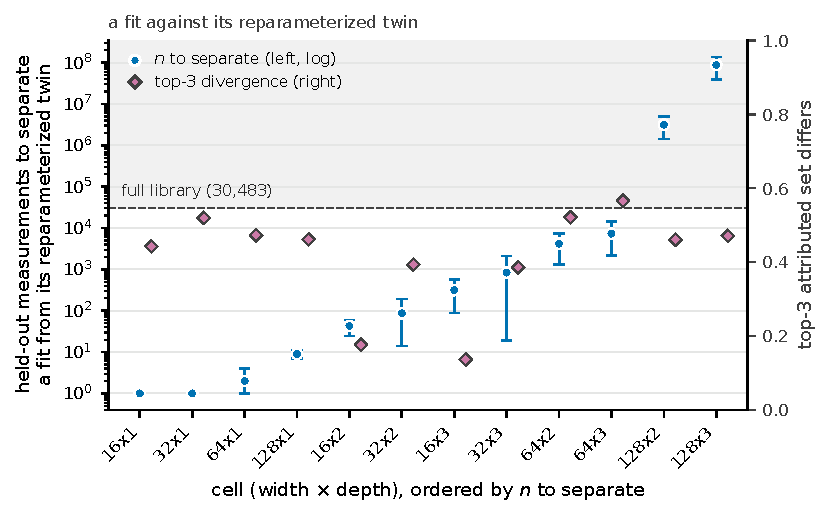
\includegraphics[width=0.85\linewidth]{figures/figA_twin_separability.pdf}
\caption{Separability and top-3 divergence for \textbf{a fit against its own reparameterized twin} --- \emph{not} for independently trained pairs. This is the separation experiment of the table above, and it is a different population from the one the main text figures describe: there, two models are trained independently and filtered to those the held-out data cannot tell apart; here, one fit is compared against a construction of itself. The two populations disagree substantially about how often the top-3 attributed set differs, so the numbers are not interchangeable and neither figure should be read as evidence for the other. Left axis logarithmic, spanning nine decades; the dashed line is the full library.}
\label{gen:twin}
\end{figure}

\section{Protocol}
\label{gen:protocol}

\paragraph{Split rule.}
Every experiment uses the same seeded split. For seed $k$, a \texttt{torch.Generator} is seeded with $1{,}000{,}003 + k$ and \texttt{torch.randperm}$(n)$ is drawn; the first 3000 indices are the fit split and the remaining 1000 are held out, from $n = 4000$ sequences. The split is therefore a deterministic function of the seed, identical across cells and across architectures within a seed, and the held-out indices are written into the run directory. Held-out points contribute nothing to any gradient.

\paragraph{Learning-rate ladder and selection.}
The ladder is learning rate over [0.01, 0.003, 0.001, 0.0003], selected once per cell and shared by all models in it. In the occurrence grid, ``no model selection: every trained model is kept and enters the pairwise analysis''. In the separation grid, ``pilot on the fit split's training loss''. The distinction matters for reading the two grids: the occurrence analysis is pairwise over all trained models, so discarding any model would bias the pair population it measures.

\paragraph{Epoch budget and seeds.}
Every cell in both grids is trained for 1,200 epochs (1,200 full-batch gradient steps), identical across width and depth so that capacity rather than budget separates the cells. Both grids use 10 seeds (0, 1, 2, 3, 4, 5, 6, 7, 8, 9), and every reported number is a mean over those seeds with a 95\% bootstrap confidence interval.

\paragraph{Tuning budget actually spent.}
Read from \texttt{tuning\_budget.json} in each run directory. The occurrence run records 12 entries, 4 configurations each, 48 configurations in total; the separation run records 12 entries, 4 each, 48 in total. The search space is the learning-rate ladder alone: no architecture, optimizer, initialization or budget search was performed, and no baseline received a larger budget than the method.

\paragraph{Configuration.}
The full resolved configuration is committed as \texttt{config.yaml} inside each run directory, alongside an \texttt{environment.lock} recording the interpreter and package versions the run actually used.

\section{Noise model derivation}
\label{gen:noise}

$Z$ requires an observation-noise scale. This library supplies one rather than needing an assumption, and the derivation is given here because the choice of count model changes $Z$ by orders of magnitude.

\paragraph{The phenotype is affine in a log count ratio.}
Each sequence carries two count pools, $\mathrm{ex}$ and $\mathrm{tot}$. Regressing the phenotype $y$ on $\log_{10}(\mathrm{ex}/\mathrm{tot})$ over the full library gives slope $0.9331$ $[0.9314, 0.9345]$ across seeds, and $r = 0.990$ over the full $30{,}483$-sequence library. The relationship is tight enough that the count ratio, not the phenotype, is the quantity whose noise must be modelled.

\paragraph{Why Poisson and not binomial.}
The two pools are \emph{not} numerator and denominator of a proportion. Over the committed library, $\mathrm{ex}$ exceeds $\mathrm{tot}$ in $4.9\%$ of rows, with ratios as large as $20.9$, and $\mathrm{ex} = 0$ in $11.4\%$ of rows. A binomial model is therefore not merely inefficient but undefined on roughly one row in twenty: $p = \mathrm{ex}/\mathrm{tot} \ge 1$ there, so the binomial variance $p(1-p)/\mathrm{tot}$ is zero or negative.

\paragraph{Delta method.}
Treating both pools as independent Poisson variates and applying the delta method to the log of their ratio,
\begin{equation}
\operatorname{var}\!\left(\log_{10} R\right) = \frac{1}{\ln(10)^2}\left(\frac{1}{\mathrm{ex}} + \frac{1}{\mathrm{tot}}\right),
\qquad
\mathrm{sd}(y_i) = |a|\,\frac{\sqrt{1/\mathrm{ex}_i + 1/\mathrm{tot}_i}}{\ln 10},
\end{equation}
with $a$ the fitted slope and a half-count continuity correction applied to both pools, which also covers the rows with $\mathrm{ex} = 0$. In the standardized units the models see, the median of this quantity is $0.3114$ $[0.3051, 0.3194]$.

\paragraph{The diagnostic that surfaced the binomial failure.}
The separation test weights points by $1/\sigma_i^2$, so a point assigned near-zero noise dominates the statistic. Under a binomial model a near-saturated sequence receives exactly that. The symptom was a weight distribution with a mean far above its median and a required sample size that collapsed to zero for every cell --- an implausible answer that is what prompted the check. Under the committed Poisson log-ratio model the mean of $1/\sigma^2$ is $3.0$ times its median, a heavy but unremarkable tail, and $Z$ becomes finite and cell-dependent. An unexamined count model would have reported that no data at all is needed to separate the fits.

We deliberately do not quote a magnitude for the binomial inflation. That model was replaced before the first commit of the separation experiment, so its exact variance form is not in the repository and the figure cannot be regenerated from committed code. What \emph{is} reproducible from the committed library is the structural defect above --- $p \ge 1$ on $4.9\%$ of rows, hence zero or negative binomial variance --- together with the Poisson ratio of $3.0$. Both were re-derived from the committed $30{,}483$-row library while preparing this appendix and agree with the recorded values.

\paragraph{$Z$ is a lower bound.}
This models sequencing noise only. Library preparation and biological variation add more, so the true noise is larger and the required sample size larger still. Every $Z$ in this paper should be read as ``at least this many''.

\section{The vacuous ceiling, in full}
\label{gen:ceiling}

\paragraph{The defect.}
The held-out closure experiment (run \texttt{20260829T181937Z\_b2951ae\_9fdd4067}, git \texttt{b2951ae}) reported that no cell contains the reparameterized twin, on the strength of a ceiling control that does not do the work it appears to do. Its refit path, \texttt{closure\_heldout.refit\_on\_split}, loads the reference weights, then evaluates the loss and snapshots the best iterate \emph{before} entering the optimisation loop. For the null target --- which is the reference's own latent --- the refit therefore begins at the answer. The measured initial loss is $6.7 \times 10^{-19}$, already below the $10^{-10}$ early-stop tolerance, so the loop breaks on its first iteration and returns the reference unchanged.

A held-out $R^2$ of $1.000000$ on that target is arithmetic, not evidence. It establishes that Adam does not wander away from a perfect solution. It does not establish that the refit can \emph{find} a solution it does not start at, which is the capability the containment conclusion depends on. Best-iterate selection is what makes the failure silent: because the initial state is already the best iterate ever seen, no subsequent step can displace it, and the procedure reports a perfect score without having searched.

\paragraph{The control that replaced it.}
Run \texttt{20260829T191427Z\_94dd5a2\_2267b74e}, git \texttt{94dd5a2}, config \texttt{2267b74e}, 10 seeds. The null target is refit \emph{without} warm-starting from the reference, from a cold random initialization. The target is known to be in the class, since the reference realises it, so this asks only whether the optimiser can travel to it. Mean initial loss across cells confirms the refit no longer begins at the answer.

\begin{table}[h]
\centering
\small
\begin{tabular}{llll}
\toprule
width & depth & cold-start null, held-out $R^2$ & warm warp refit, held-out $R^2$ \\
\midrule
16 & 1 & 0.9988 \small[0.9982, 0.9993] & 0.9748 \small[0.9669, 0.9809] \\
16 & 2 & 0.9476 \small[0.9244, 0.9703] & 0.9935 \small[0.9895, 0.9962] \\
16 & 3 & 0.7763 \small[0.6820, 0.8589] & 0.9959 \small[0.9921, 0.9986] \\
32 & 1 & 0.9994 \small[0.9990, 0.9997] & 0.9749 \small[0.9708, 0.9789] \\
32 & 2 & 0.8258 \small[0.7303, 0.9103] & 0.9463 \small[0.9185, 0.9724] \\
32 & 3 & 0.5626 \small[0.4404, 0.6891] & 0.9404 \small[0.9151, 0.9643] \\
64 & 1 & 0.9971 \small[0.9955, 0.9984] & 0.9804 \small[0.9696, 0.9893] \\
64 & 2 & 0.7122 \small[0.5620, 0.8561] & 0.9236 \small[0.8929, 0.9532] \\
64 & 3 & 0.4501 \small[0.3529, 0.5575] & 0.9034 \small[0.8879, 0.9186] \\
128 & 1 & 0.9969 \small[0.9962, 0.9975] & 0.9885 \small[0.9868, 0.9900] \\
128 & 2 & 0.8997 \small[0.8316, 0.9529] & 0.9575 \small[0.9381, 0.9734] \\
128 & 3 & 0.5328 \small[0.4000, 0.6714] & 0.9247 \small[0.9108, 0.9394] \\
\bottomrule
\end{tabular}
\caption{The ceiling that requires search. The cold-start column is an upper bound on what this procedure can say about any target, because its target is in the class by construction. Mean cold-start initial loss ranges from $1.826$ to $2.093$, against $6.7 \times 10^{-19}$ for the warm-started control it replaces.}
\end{table}

\paragraph{What the control shows.}
Read by depth: at depth 1 the worst-cell cold-start null reaches $0.9969$ against $0.9748$ for the warm warp refit, so the ceiling sits above the measurement; at depth 2 the worst-cell cold-start null reaches $0.7122$ against $0.9236$ for the warm warp refit, so the ceiling sits below the measurement; at depth 3 the worst-cell cold-start null reaches $0.4501$ against $0.9034$ for the warm warp refit, so the ceiling sits below the measurement.

At depth 1 the ceiling sits above the measurement, so the comparison is valid there and the warp target is genuinely not reached as well as an in-class one. At depths 2 and 3 the ranking inverts: the warm-started warp refit scores \emph{higher} than a cold-started refit to a target guaranteed to be in the class. That is initialization dominating the result, and no conclusion about what the class contains can be drawn at those depths. The configured pass threshold is $0.999$, and 11 of 12 cells fall below it.

The honest reading is therefore narrower than the original claim: the refit procedure did not find a member of the class equal to the twin. That is consistent with no such member existing, and equally consistent with one existing that the optimiser failed to reach.

\section{Reproducibility}
\label{gen:repro}

\paragraph{Repository.}
\url{https://github.com/shadi97kh/CERTGNN}. Every experiment writes a directory under \texttt{results/runs/} named \texttt{<timestamp>\_<gitsha>\_<confighash>}, containing the resolved \texttt{config.yaml}, an \texttt{environment.lock}, a \texttt{meta.json} recording the git SHA and whether the tree was dirty, a \texttt{tuning\_budget.json}, per-seed JSON, and the aggregated \texttt{results.json}. Every number in this paper is read from one of those files by a generator script; none is transcribed by hand.

\begin{table}[h]
\centering
\small
\begin{tabular}{lllll}
\toprule
experiment & run directory & git SHA & config hash & seeds \\
\midrule
\texttt{closure\_heldout} & \texttt{\scriptsize 20260829T181937Z\_b2951ae\_9fdd4067} & \texttt{b2951ae} & \texttt{9fdd4067} & 10 \\
\texttt{closure\_search} & \texttt{\scriptsize 20260829T191427Z\_94dd5a2\_2267b74e} & \texttt{94dd5a2} & \texttt{2267b74e} & 10 \\
\texttt{occurrence} & \texttt{\scriptsize 20260830T002223Z\_6f98de3\_6e25cf7d} & \texttt{6f98de3} & \texttt{6e25cf7d} & 10 \\
\texttt{separation} & \texttt{\scriptsize 20260830T030657Z\_972496a\_5da8cb38} & \texttt{972496a} & \texttt{5da8cb38} & 10 \\
\bottomrule
\end{tabular}
\caption{Every run directory cited in this paper. A run recorded against a dirty tree is marked; none of the runs cited here is.}
\end{table}

\paragraph{Pre-registration.}
\texttt{PREREGISTRATION.md} records the claims, the gate thresholds and the falsification conditions. It was committed on 2026-08-26 in \texttt{6d0719a} and has never been amended: its git history contains 1 commit. The earliest committed run directory dates from 2026-08-29, so the pre-registration predates every result reported here, and this is checkable from the repository history rather than asserted.

Amendment is additionally blocked by a tool-level pre-write hook, \texttt{scripts/hooks/protect\_prereg.sh}, registered as a \texttt{PreToolUse} hook. The hook matches the \emph{target path} of a write and refuses any edit whose destination is \texttt{PREREGISTRATION.md}, including shell redirections, \texttt{sed -i}, \texttt{mv}, \texttt{cp} and \texttt{rm} aimed at it. It deliberately does not fire on files that merely mention the pre-registration by name, an earlier behaviour that produced false positives and trained bypasses. The guard is inert until results exist, so the first write is permitted and every subsequent one is not. We state the mechanism precisely because it is a hook in the authoring environment rather than a server-side or \texttt{pre-commit} enforcement: it constrains the workflow that produced this paper, and the durable evidence is the single-commit git history above.


\end{document}